\section{R$_2$ in Pure QED}
\label{sec:pureQED} 
\subsection{2-point functions}
{\bf Photon self-energy} \\
\begin{align*}
\begin{gathered}
\feynmandiagram [layered layout, horizontal=b to c] {
	a [particle=\(\alpha\)] -- [photon, momentum=\(p_1\)] b
	  -- [fermion, half left, looseness=1.5, momentum=\(p_1+q\)] c
	  -- [fermion, half left, looseness=1.5, momentum=\(q\)] b,
	c -- [photon, momentum=\(p_1\)] d [particle=\(\beta\)] ,
};
\end{gathered} \qquad
& =\int\frac{d^dq}{\left( 2\pi \right)^d} \left( -1 \right) \mathrm{Tr} \lbr ie \gamma^{\alpha} \frac{i \left( \fsl{p}_1+\fsl{q}+m \right)}{\left( p_1+q \right)^2 - m^2} ie \gamma^{\beta} \frac{i \left( \fsl{q}+m \right)}{q^2 - m^2} \rbr & \\
& \equiv \int\frac{d^dq}{\left( 2\pi \right)^d} \frac{\bar{N}}{\bar{D}_1\bar{D}_0} &
\end{align*}

From now on bared quantities are $d$-dimensional, the quantities with a tilde $\epsilon$-dimensional and the normal momenta and gamma matrices 4-dimensional. 
\begin{equation*}
\bar{N} (\bar{q}) = - e^2 \ \mathrm{Tr} \lbr \bar{\gamma}^{\alpha} \left( \bar{\fsl{p}}_1 + \bar{\fsl{q}} + m \right) \bar{\gamma}^{\beta} \left( \bar{\fsl{q}} + m \right) \rbr = - e^2 \ \mathrm{Tr} \lbr \gamma^{\alpha} \left( \fsl{p}_1 + \fsl{q} + m \right) \gamma^{\beta} \left( \fsl{q} + m \right) + \gamma^{\alpha} \tilde{\fsl{q}} \gamma^{\beta} \tilde{\fsl{q}} \rbr \equiv N + \tilde{N}
\end{equation*}

\begin{equation*}
\tilde{N} = -e^2 \ \mathrm{Tr} \lbr \gamma^{\alpha} \tilde{\fsl{q}} \gamma^{\beta} \tilde{\fsl{q}} \rbr \overset{\lbr \gamma^{\mu} , \tilde{\gamma}^{\nu} \rbr = 0}{=} 4 e^2 \tilde{q}^2 g^{\alpha\beta}
\end{equation*}

\begin{equation}
\label{eqn:R2photon}
R_2^{\gamma\gamma} = \frac{1}{\left( 2\pi \right) ^4} \int d^d\bar{q} \frac{\tilde{N}}{\bar{D}_1\bar{D}_0} = \frac{4e^2}{16\pi^4} \underbrace{\int d^d\bar{q} \frac{\tilde{q}^2}{\bar{D}_1\bar{D}_0}}_{-i\frac{\pi}{2} \left( m^2 - p_1^2/3 \right)} = \frac{-ie^2}{8\pi^2} g^{\alpha\beta} \left( 2m^2 -\frac{p_1^2}{3} \right)
\end{equation}
\\

{\bf Electron self-energy} \\
\begin{align*}
\begin{gathered}
\feynmandiagram [layered layout, horizontal=b to c] {
	a -- [fermion, momentum=\(p_1\)] b,
	c -- [photon, half left, looseness=1.5, momentum=\(q\)] b,
	b -- [fermion, momentum=\(p_1+q\)] c,
	c -- [fermion, momentum=\(p_1\)] d,
};
\end{gathered} \qquad
& =\int\frac{d^dq}{\left( 2\pi \right)^d} ie \gamma^{\alpha} \frac{i \left( \fsl{p}_1+\fsl{q}+m \right)}{\left( p_1+q \right)^2 - m^2} ie \gamma^{\beta} \frac{-i g_{\alpha\beta}}{q^2} =\int\frac{d^dq}{\left( 2\pi \right)^d} \left( -e^2 \right) \gamma^{\alpha} \frac{\left( \fsl{p}_1+\fsl{q}+m \right)}{\left( p_1+q \right)^2 - m^2} \gamma_{\alpha} \frac{1}{q^2} & \\
& \equiv \int\frac{d^dq}{\left( 2\pi \right)^d} \frac{\bar{N}}{\bar{D}_1\bar{D}_0} &
\end{align*}

\begin{equation*}
\bar{N} (\bar{q}) = \left( -e^2 \right) \bar{\gamma}^{\alpha} \left( \bar{\fsl{p}}_1 + \bar{\fsl{q}} + m \right) \bar{\gamma}_{\alpha} = -e^2 \lbr \gamma^{\alpha} \left( \bar{\fsl{p}}_1 + \bar{\fsl{q}} + m \right) \gamma_{\alpha} + \tilde{\gamma}^{\alpha} \left( \bar{\fsl{p}}_1 + \bar{\fsl{q}} + m \right) \tilde{\gamma}_{\alpha} + \gamma^{\alpha} \tilde{\fsl{q}} \gamma_{\alpha} + \tilde{\gamma}^{\alpha} \tilde{\fsl{q}} \tilde{\gamma}_{\alpha} \rbr \equiv N + \tilde{N}
\end{equation*}

\begin{equation*}
\tilde{N} = -e^2 \lbr \tilde{\gamma}^{\alpha} \left( \bar{\fsl{p}}_1 + \bar{\fsl{q}} + m \right) \tilde{\gamma}_{\alpha} + \gamma^{\alpha} \tilde{\fsl{q}} \gamma_{\alpha} + \tilde{\gamma}^{\alpha} \tilde{\fsl{q}} \tilde{\gamma}_{\alpha} \rbr = -e^2 \lbr - \underbrace{\tilde{\gamma}^{\alpha} \tilde{\gamma}_{\alpha}}_{= \epsilon} \left( \bar{\fsl{p}}_1 + \bar{\fsl{q}} - m \right) - \underbrace{\gamma^{\alpha} \gamma_{\alpha}}_{=4} \tilde{\fsl{q}} + \tilde{\gamma}^{\alpha} \tilde{\fsl{q}} \tilde{\gamma}_{\alpha} \rbr
\end{equation*}
\begin{align*}
R_2^{\mathrm{ee}} & = \frac{1}{\left( 2\pi \right) ^4} \int d^d\bar{q} \frac{\tilde{N}}{\bar{D}_1\bar{D}_0} = \frac{-e^2}{\left( 2\pi \right) ^4} \int d^d\bar{q} \frac{1}{\bar{D}_1\bar{D}_0} \left( -\epsilon \left( \fsl{p}_1 + \fsl{q} - m \right) + \underbrace{\tilde{\fsl{q}} \left( \ldots \right)}_{=0} \right) = & \\ 
& = \frac{e^2}{\left( 2\pi \right) ^4} \lbr \underbrace{\int d^d\bar{q} \frac{\epsilon \left( \fsl{p}_1 - m \right)}{\bar{D}_1\bar{D}_0}}_{=-2\epsilon \frac{i \pi^2}{\epsilon}  \left( \fsl{p}_1 -m \right)}  + \underbrace{\int d^d\bar{q} \frac{\epsilon \fsl{q}}{\bar{D}_1\bar{D}_0}}_{=\epsilon \frac{i\pi^2}{\epsilon} \fsl{p}_1} \rbr = \frac{e^2}{\left( 2\pi \right) ^4} \epsilon \frac{i\pi^2}{\epsilon} \left( \left( -2 \right) \left( \fsl{p}_1 - m \right) + \fsl{p}_1 \right) = \frac{-ie^2}{16 \pi^2}  \left( \fsl{p}_1 - 2m \right) & \numberthis \label{eqn:R2ee}
\end{align*}


\subsection{3-point functions}
\begin{align*}
\begin{gathered}
\feynmandiagram [horizontal=i1 to v2] {
	i1 [particle=\mu] -- [photon, momentum=\(p_2-p_1\)] v2,
	f1 -- [fermion, momentum=\(p_1\)] v1
	   -- [fermion, momentum=\(p_1+q\)] v2
	   -- [fermion, momentum=\(p_2+q\)] v3
	   -- [fermion, momentum=\(p_2\)] f3,
	v3 -- [boson, momentum=\(q\)] v1, 
};
\end{gathered} \qquad
& =\int\frac{d^dq}{\left( 2\pi \right)^d} ie \gamma^{\beta} \frac{i \left( \fsl{p}_1+\fsl{q}+m \right)}{\left( p_1+q \right)^2 - m^2} ie \gamma^{\mu} \frac{i \left( \fsl{p}_2 + \fsl{q}+m \right)}{\left( p_2 + q \right)^2 - m^2} ie \gamma^{\alpha} \frac{-ig_{\alpha\beta}}{q^2} & \\
& \equiv \int\frac{d^dq}{\left( 2\pi \right)^d} \frac{\bar{N}}{\bar{D}_1\bar{D}_2\bar{D}_0} &
\end{align*}

\begin{align*}
\bar{N} (\bar{q}) & = e^3 \lbr \bar{\gamma}^{\beta} \left( \bar{\fsl{p}}_1 + \bar{\fsl{q}} + m \right) \bar{\gamma}^{\mu} \left( \bar{\fsl{p}}_2 + \bar{\fsl{q}} + m \right) \bar{\gamma}_{\beta} \rbr = e^3 \lbr \gamma^{\beta} \left( \fsl{p}_1 + \fsl{q} + m \right) \gamma^{\mu} \left( \fsl{p}_2 + \fsl{q} + m \right) \gamma_{\beta} + \right. & \\
& \left. + \tilde{\gamma}^{\beta} \left( \fsl{p}_1 + \fsl{q} + m \right) \gamma^{\mu} \left( \fsl{p}_2 + \fsl{q} + m \right) \tilde{\gamma}_{\beta} + \underbrace{\gamma^{\beta} \tilde{\fsl{q}} \gamma^{\mu} \tilde{\fsl{q}} \gamma_{\beta}}_{\equiv \ \circled{1}} + \underbrace{\tilde{\gamma}^{\beta} \tilde{\fsl{q}} \gamma^{\mu} \tilde{\fsl{q}} \tilde{\gamma}_{\beta}}_{\equiv \ \circled{2}}  \rbr \equiv N + \tilde{N} &
\end{align*}
\begin{equation*}
\circled{1} = \tilde{q}_{\rho}\tilde{q}_{\sigma} \gamma^{\beta} \tilde{\gamma}^{\rho} \gamma^{\mu} \tilde{\gamma}^{\sigma} \gamma_{\beta} = \tilde{q}_{\rho}\tilde{q}_{\sigma} \left( -1 \right)^3 \tilde{\gamma}^{\rho} \tilde{\gamma}^{\sigma} \gamma^{\beta} \gamma^{\mu} \gamma_{\beta} = -2\tilde{\fsl{q}}\tilde{\fsl{q}}\gamma^{\mu} = -2 \tilde{q}^2 \gamma^{\mu}
\end{equation*}
\begin{equation*}
\circled{2} = \tilde{q}_{\rho}\tilde{q}_{\sigma} \tilde{\gamma}^{\beta} \tilde{\gamma}^{\rho} \gamma^{\mu} \tilde{\gamma}^{\sigma} \tilde{\gamma}_{\beta} = \tilde{q}_{\rho}\tilde{q}_{\sigma} \left( -1 \right)^2 \gamma^{\mu} \tilde{\gamma}^{\beta} \tilde{\gamma}^{\rho} \tilde{\gamma}^{\sigma} \tilde{\gamma}_{\beta} = \tilde{q}^2 \gamma^{\mu} \tilde{\gamma}^{\beta} \tilde{\gamma}_{\beta} = \epsilon \tilde{q}^2 \gamma^{\mu}
\end{equation*}

\begin{equation*}
\tilde{N} = - \epsilon \left( \fsl{p}_1 + \fsl{q} - m \right) \gamma^{\mu} \left( \fsl{p}_2 + \fsl{q} - m \right) - \left( 2 - \epsilon \right) \tilde{q}^2 \gamma^{\mu}
\end{equation*}
\begin{align*}
R_2^{\gamma\mathrm{ee}} = & \frac{1}{\left( 2\pi \right) ^4} \int d^d\bar{q} \frac{\tilde{N}}{\bar{D}_0 \bar{D}_1 \bar{D}_2} = \frac{1}{\left( 2\pi \right) ^4} \int d^d\bar{q} \frac{e^3}{\bar{D}_0 \bar{D}_1 \bar{D}_2} \lbr -\epsilon \left( \fsl{p}_1 + \fsl{q} - m \right) \gamma^{\mu} \left( \fsl{p}_2 + \fsl{q} - m \right) - \left( 2 - \epsilon \right) \tilde{q}^2 \gamma^{\mu} \rbr = & \\
& = \frac{e^3}{\left( 2\pi \right) ^4} \int d^d\bar{q} \frac{1}{\bar{D}_0 \bar{D}_1 \bar{D}_2} \lbr -\epsilon \fsl{q}\gamma^{\mu}\fsl{q} - \left( 2 - \epsilon \right) \tilde{q}^2 \gamma^{\mu} \rbr = \frac{e^3}{\left( 2\pi \right) ^4} \lbr -\epsilon \gamma^{\alpha}\gamma^{\mu}\gamma^{\beta} \left( \frac{-i\pi^2}{2\epsilon} g_{\alpha\beta} \right) - \frac{-i\pi^2}{2} \left(2 - \epsilon \right) \gamma^{\mu} \rbr = & \\
& = \frac{e^3}{\left( 2\pi \right) ^4} \frac{i \pi^2}{2} \lbr \gamma^{\alpha}\gamma^{\mu}\gamma_{\alpha} - 2\gamma^{\mu} + O(\epsilon) \rbr = \frac{-ie^3}{8\pi^2} \gamma^{\mu} & \numberthis \label{eqn:R2photonee}
\end{align*}

There is one more 3-point function at the 1-loop level which is allowed by the Feynman rules: the 3-point function with only photons as external particles. But it does not contribute to $R_2$ which we will show now. Because of the symmetry of the 3-point function there are 2 contributing diagrams
\begin{align*}
\begin{gathered}
\feynmandiagram [small, horizontal=i1 to v] {
	i1 [particle=\alpha] -- [photon, momentum=\(-p_1-p_2\)] v [crossed dot],
	i2 [particle=\beta] -- [photon, momentum=\(p_1\)] v,
	i3 [particle=\gamma] -- [photon, momentum=\(p_2\)] v,
};
\end{gathered}
\quad = \quad  
\begin{gathered}
\feynmandiagram [horizontal=i1 to v1] {
	i1 [particle=\alpha] -- [photon, momentum=\(-p_1-p_2\)] v1,
	i3 [particle=\gamma] -- [photon, momentum=\(p_2\)] v3,
	i2 [particle=\beta] -- [photon, momentum=\(p_1\)] v2,
	v3 -- [fermion, momentum'=\(q\)] v2
	   -- [fermion, momentum'=\(p_1+q\)] v1
	   -- [fermion, momentum'=\(q-p_2\)] v3,
};
\end{gathered}
\quad + \quad
\begin{gathered}
\feynmandiagram [horizontal=i1 to v1] {
	i1 [particle=\alpha] -- [photon, momentum=\(-p_1-p_2\)] v1,
	i3 [particle=\gamma] -- [photon, momentum=\(p_2\)] v3,
	i2 [particle=\beta] -- [photon, momentum=\(p_1\)] v2,
	v2 -- [fermion, momentum=\(q\)] v3
	   -- [fermion, momentum=\(p_2+q\)] v1
	   -- [fermion, momentum=\(q-p_1\)] v2,
};
\end{gathered}
\end{align*}

We only calculate the first diagram and then symmetrize the result with $p_1 \leftrightarrow p_2$, $\beta \leftrightarrow \gamma$. Evaluating the first diagram gives
\begin{align*}
\begin{gathered}
\feynmandiagram [horizontal=i1 to v1] {
	i1 [particle=\alpha] -- [photon, momentum=\(-p_1-p_2\)] v1,
	i3 [particle=\gamma] -- [photon, momentum=\(p_2\)] v3,
	i2 [particle=\beta] -- [photon, momentum=\(p_1\)] v2,
	v3 -- [fermion, momentum'=\(q\)] v2
	   -- [fermion, momentum'=\(p_1+q\)] v1
	   -- [fermion, momentum'=\(q-p_2\)] v3,
};
\end{gathered}
\qquad
& =\int\frac{d^dq}{\left( 2\pi \right)^d} \Tr \lbr ie\gamma^{\beta} \frac{i \left( \fsl{q} + m \right)}{q^2 - m^2} ie \gamma^{\gamma} \frac{i \left( \fsl{q} - \fsl{p}_2 + m \right)}{\left( q- p_2 \right) -m^2} ie \gamma^{\alpha} \frac{i \left( \fsl{q} + \fsl{p}_1 + m \right)}{\left( q + p_1 \right) -m^2} \rbr =  & \\
& = \int\frac{d^dq}{\left( 2\pi \right)^d} e^3 \Tr \lbr \gamma^{\beta} \frac{\left( \fsl{q} + m \right)}{q^2 - m^2} \gamma^{\gamma} \frac{\left( \fsl{q} - \fsl{p}_2 + m \right)}{\left( q- p_2 \right) -m^2} \gamma^{\alpha} \frac{\left( \fsl{q} + \fsl{p}_1 + m \right)}{\left( q + p_1 \right) -m^2} \rbr = & \\
& \equiv \int\frac{d^dq}{\left( 2\pi \right)^d} \frac{\bar{N}}{\bar{D}_1\bar{D}_2\bar{D}_0} &
\end{align*}

\begin{align*}
\bar{N} (\bar{q}) & = e^3 \Tr \lbr \bar{\gamma}^{\beta} \left( \bar{\fsl{q}} + m \right) \bar{\gamma}^{\gamma} \left( \bar{\fsl{q}} - \bar{\fsl{p}}_2 + m \right) \bar{\gamma}^{\alpha} \left( \bar{\fsl{q}} + \bar{\fsl{p}}_1 + m \right) \rbr = & \\
& = e^3 \Tr \lbr \gamma^{\beta} \left( \fsl{q} + m \right) \gamma^{\gamma} \left( \fsl{q} - \fsl{p}_2 + m \right) \gamma^{\alpha} \left( \fsl{q} + \fsl{p}_1 + m \right) +  \gamma^{\beta} \left( \fsl{q} + \tilde{\fsl{q}} + m \right) \gamma^{\gamma} \left( \fsl{q} + \tilde{\fsl{q}} - \fsl{p}_2 + m \right) \gamma^{\alpha} \left( \fsl{q} + \tilde{\fsl{q}} + \fsl{p}_1 + m \right) \rbr = & \\
& \equiv N + \tilde{N} &
\end{align*}

\begin{align*}
\tilde{N} & = e^3 \Tr \lbr \gamma^{\beta} \left( \fsl{q} + \tilde{\fsl{q}} + m \right) \gamma^{\gamma} \left( \fsl{q} + \tilde{\fsl{q}} - \fsl{p}_2 + m \right) \gamma^{\alpha} \left( \fsl{q} + \tilde{\fsl{q}} + \fsl{p}_1 + m \right) \rbr = & \\
& = e^3 \Tr \lbr \gamma^{\beta} \fsl{q} \gamma^{\gamma} \tilde{\fsl{q}} \gamma^{\alpha} \tilde{\fsl{q}} + \gamma^{\beta} \tilde{\fsl{q}} \gamma^{\gamma} \fsl{q} \gamma^{\alpha} \tilde{\fsl{q}} + \gamma^{\beta} \tilde{\fsl{q}} \gamma^{\gamma} \tilde{\fsl{q}} \gamma^{\alpha} \fsl{q} + \gamma^{\beta} \tilde{\fsl{q}} \gamma^{\gamma} \left( - \fsl{p}_2 \right) \gamma^{\alpha} \tilde{\fsl{q}} + \gamma^{\beta} \tilde{\fsl{q}} \gamma^{\gamma} \tilde{\fsl{q}} \gamma^{\alpha} \fsl{p}_1 \rbr = & \\
& = - 4e^3 \tilde{q}^2 \lbr q_{\mu} \left[ \left( g^{\beta\mu}g^{\gamma\alpha} - g^{\beta\gamma}g^{\mu\alpha} + g^{\beta\alpha}g^{\mu\gamma} \right) + \left( g^{\beta\gamma}g^{\alpha\mu} - g^{\beta\mu}g^{\gamma\alpha} + g^{\beta\alpha}g^{\mu\gamma} \right) + \left( g^{\beta\gamma}g^{\mu\alpha} - g^{\beta\alpha}g^{\mu\gamma} + g^{\beta\mu}g^{\alpha\gamma} \right) \right] + \right. & \\ 
& \left. + p_{1\mu} \left( g^{\beta\gamma}g^{\alpha\mu} - g^{\beta\alpha}g^{\gamma\mu} + g^{\beta\mu}g^{\alpha\gamma} \right) - p_{2\mu} \left( g^{\beta\gamma}g^{\mu\alpha} - g^{\beta\mu}g^{\alpha\gamma} + g^{\alpha\beta}g^{\gamma\mu} \right) \rbr = & \\
& = -4e^3 \tilde{q}^2 \lbr q^{\beta}g^{\alpha\gamma} + q^{\gamma}g^{\alpha\beta} + q^{\alpha}g^{\beta\gamma} + p_1^{\alpha}g^{\beta\gamma} - p_1^{\gamma}g^{\alpha\beta} + p_1^{\beta}g^{\alpha\gamma} - p_2^{\alpha}g^{\beta\gamma} + p_2^{\beta}g^{\alpha\gamma} - p_2^{\gamma}g^{\alpha\beta} \rbr &
\end{align*}

This gives for the $R_2$ contribution of the first diagram
\begin{align*}
R_2^1 & = \frac{1}{\left( 2\pi \right)^4} \int d^d\bar{q} \frac{\tilde{N}}{\bar{D}_1\bar{D}_{-2}\bar{D}_0} = & \\
& = \frac{-4e^3}{\left( 2\pi \right)^4} \int d^d \bar{q} \frac{1}{\bar{D}_1\bar{D}_{-2}\bar{D}_0} \lbr \tilde{q}^2q^{\beta}g^{\alpha\gamma} + \tilde{q}^2q^{\gamma}g^{\alpha\beta} + \tilde{q}^2q^{\alpha}g^{\beta\gamma} + \tilde{q}^2 \left[ \left( p_1 - p_2 \right)^{\alpha} g^{\beta\gamma} + \left( p_1 + p_2 \right)^{\beta} g^{\alpha\gamma} - \left( p_1 + p_2 \right)^{\gamma} g^{\alpha\beta} \right] \rbr = & \\
& = \frac{-4e^3}{\left( 2\pi \right)^4} \lbr \frac{i\pi^2}{6} \left[ \left( p_1-p_2 \right)^{\beta}g^{\alpha\gamma} + \left( p_1-p_2 \right)^{\gamma}g^{\alpha\beta} + \left( p_1-p_2 \right)^{\alpha}g^{\beta\gamma} \right] - \frac{i\pi^2}{2} \left[ \left( p_1-p_2 \right)^{\alpha} g^{\beta\gamma} + \left( p_1+p_2 \right)^{\beta} g^{\alpha\gamma} + \right. \right. & \\
& \left. \left. - \left( p_1+p_2 \right)^{\gamma} g^{\alpha\beta} \right] \rbr = & \\
& = \frac{-4e^3}{\left( 2\pi \right)^4} \lbr g^{\alpha\beta} \left[ \frac{i\pi^2}{6} \left( p_1-p_2 \right)^{\gamma} + \frac{i\pi^2}{2} \left( p_1+p_2 \right)^{\gamma} \right] + g^{\beta\gamma} \left[ \frac{i\pi^2}{6} \left( p_1-p_2 \right)^{\alpha} - \frac{i\pi^2}{2} \left( p_1-p_2 \right)^{\alpha} \right] + \right. & \\
& \left. + g^{\alpha\gamma} \left[ \frac{i\pi^2}{6} \left( p_1-p_2 \right)^{\beta} - \frac{i\pi^2}{2} \left( p_1+p_2 \right)^{\beta} \right] \rbr &
\end{align*}

\begin{align*}
R_2^2 & = R_1^2(p_1 \leftrightarrow p_2, \ \beta \leftrightarrow \gamma) = & \\
& = \frac{-4e^3}{\left( 2\pi \right)^4} \lbr g^{\alpha\gamma} \left[ \frac{i\pi^2}{6} \left( p_2-p_1 \right)^{\beta} + \frac{i\pi^2}{2} \left( p_2+p_1 \right)^{\beta} \right] + g^{\beta\gamma} \left[ \frac{i\pi^2}{6} \left( p_2-p_1 \right)^{\alpha} - \frac{i\pi^2}{2} \left( p_2-p_1 \right)^{\alpha} \right] + \right. & \\
& \left. + g^{\alpha\beta} \left[ \frac{i\pi^2}{6} \left( p_2-p_1 \right)^{\gamma} - \frac{i\pi^2}{2} \left( p_2+p_1 \right)^{\gamma} \right] \rbr = & \\
& = \frac{-4e^3}{\left( 2\pi \right)^4} \lbr -g^{\alpha\beta} \left[ \frac{i\pi^2}{6} \left( p_1-p_2 \right)^{\gamma} + \frac{i\pi^2}{2} \left( p_1+p_2 \right)^{\gamma} \right] - g^{\beta\gamma} \left[ \frac{i\pi^2}{6} \left( p_1-p_2 \right)^{\alpha} - \frac{i\pi^2}{2} \left( p_1-p_2 \right)^{\alpha} \right] + \right. & \\
& \left. - g^{\alpha\gamma} \left[ \frac{i\pi^2}{6} \left( p_1-p_2 \right)^{\beta} - \frac{i\pi^2}{2} \left( p_1+p_2 \right)^{\beta} \right] \rbr = -R_2^1 &
\end{align*}

\begin{equation}
R_2^{3\gamma} = R_2^1 + R_2^2 = R_2^1 - R_2^1 = 0
\end{equation}

\subsection{4-point function}
For the 4-point function we have to be more careful. The 1PI contribution at the 1-loop level consists of several diagrams. They are obtained by symmetrizing the external momenta of the diagram as follows
\begin{align*}
\begin{gathered}
\feynmandiagram [small, horizontal=i1 to i2] {
	i4 [particle=\delta] -- [photon, momentum=\(p_2\)] v [crossed dot],
	i2 [particle=\beta] -- [photon, momentum=\(p_3\)] v,
	i1 [particle=\alpha] -- [photon, momentum=\(p_1\)] v,
	i3 [particle=\gamma] -- [photon, momentum=\(p_4\)] v,
};
\end{gathered}
= 2 \times \lbr
\begin{gathered}
\feynmandiagram [horizontal=i4 to i3] {
	i2 [particle=\beta] -- [photon, momentum=\(p_3\)] v2,
	i4 [particle=\delta] -- [photon, momentum=\(p_2\)] v4,
	i1 [particle=\alpha] -- [photon, momentum=\(p_1\)] v1,
	i3 [particle=\gamma] -- [photon, momentum=\(p_4\)] v3,
	v4 -- [fermion, momentum=\(q\)] v1
	   -- [fermion, momentum=\(p_1+q\)] v2
	   -- [fermion, momentum=\(q+p_1+p_3\)] v3
	   -- [fermion, momentum=\(q-p_2\)] v4,
};
\end{gathered}
\ \ + \ \ \left( \alpha \leftrightarrow \beta; \ p_1 \leftrightarrow p_3 \right) \ + \ \left( \alpha \leftrightarrow \delta; \ p_1 \leftrightarrow p_2 \right) \rbr 
\end{align*}

We only calculate one of the diagrams and do the symmetrizing with the result of our calculation, so we only have to evaluate one diagram. The first of the three diagrams gives
\begin{align*}
\begin{gathered}
\feynmandiagram [horizontal=i4 to i3] {
	i2 [particle=\beta] -- [photon, momentum=\(p_3\)] v2,
	i4 [particle=\delta] -- [photon, momentum=\(p_2\)] v4,
	i1 [particle=\alpha] -- [photon, momentum=\(p_1\)] v1,
	i3 [particle=\gamma] -- [photon, momentum=\(p_4\)] v3,
	v4 -- [fermion, momentum=\(q\)] v1
	   -- [fermion, momentum=\(p_1+q\)] v2
	   -- [fermion, momentum=\(q+p_1+p_3\)] v3
	   -- [fermion, momentum=\(q-p_2\)] v4,
};
\end{gathered}\qquad
& = \int\frac{d^dq}{\left( 2\pi \right)^d} \left( -1 \right) \mathrm{Tr} \lbr ie \gamma^{\alpha} \frac{i \left( \fsl{p}_1 + \fsl{q} + m \right)}{\left( p_1 +q \right) ^2 -m^2} ie \gamma^{\beta} \frac{i \left( \fsl{q} + \fsl{p}_3 + \fsl{p}_1 + m \right)}{\left( p_3 + p_1 +q \right) ^2 -m^2} \times \right. & \\
& \left. \times ie \gamma^{\gamma} \frac{i \left( \fsl{q} - \fsl{p}_2 + m \right)}{\left( q - p_2 \right) ^2 - m^2} ie \gamma^{\delta} \frac{i \left( \fsl{q} + m \right)}{q ^2 - m^2} \rbr \equiv \int\frac{d^dq}{\left( 2\pi \right)^d} \frac{\bar{N}}{\bar{D}_1\bar{D}_{13}\bar{D}_2\bar{D}_0} &
\end{align*}

\begin{align*}
\bar{N} (\bar{q}) & = -e^4 \mathrm{Tr} \lbr \bar{\gamma}^{\alpha} \left( \bar{\fsl{p}}_1 + \bar{\fsl{q}} + m \right) \bar{\gamma}^{\beta} \left( \bar{\fsl{q}} +  \bar{\fsl{p}}_1 + \bar{\fsl{p}}_3 + m \right) \bar{\gamma}^{\gamma} \left( \bar{\fsl{q}} - \bar{\fsl{p}}_2 + m \right) \bar{\gamma}^{\delta} \left( \bar{\fsl{q}} + m \right) \rbr = & \\
& = -e^4 \mathrm{Tr} \lbr \gamma^{\alpha} \left( \fsl{p}_1 + \fsl{q} + m \right) \gamma^{\beta} \left( \fsl{q} +  \fsl{p}_1 + \fsl{p}_3 + m \right) \gamma^{\gamma} \left( \fsl{q} - \fsl{p}_2 + m \right) \gamma^{\delta} \left( \fsl{q} + m \right) + \right. &  \\
&  \left. + \gamma^{\alpha} \tilde{\fsl{q}} \gamma^{\beta} \tilde{\fsl{q}} \gamma^{\gamma} \tilde{\fsl{q}} \gamma^{\delta} \tilde{\fsl{q}} + \gamma^{\alpha} \tilde{\fsl{q}} \gamma^{\beta} \tilde{\fsl{q}} \gamma^{\gamma} \fsl{q} \gamma^{\delta} \fsl{q}  + \gamma^{\alpha} \fsl{q} \gamma^{\beta} \tilde{\fsl{q}} \gamma^{\gamma} \tilde{\fsl{q}} \gamma^{\delta} \fsl{q} + \gamma^{\alpha} \fsl{q} \gamma^{\beta} \fsl{q} \gamma^{\gamma} \tilde{\fsl{q}} \gamma^{\delta} \tilde{\fsl{q}} + \gamma^{\alpha} \tilde{\fsl{q}} \gamma^{\beta} \fsl{q} \gamma^{\gamma} \fsl{q} \gamma^{\delta} \tilde{\fsl{q}} + \right. & \\
& \left. + \gamma^{\alpha} \tilde{\fsl{q}} \gamma^{\beta} \fsl{q} \gamma^{\gamma} \tilde{\fsl{q}} \gamma^{\delta} \fsl{q} + \gamma^{\alpha} \fsl{q} \gamma^{\beta} \tilde{\fsl{q}} \gamma^{\gamma} \fsl{q} \gamma^{\delta} \tilde{\fsl{q}} \rbr \equiv N + \tilde{N} &
\end{align*}

Where we have used that the trace of an odd number of Dirac matrices is zero. Using (..) and (..) $\tilde{N}$ can be further simplified to
\begin{align*}
\tilde{N} = & -e^4 \mathrm{Tr} \lbr \left( -1 \right)^{10} \tilde{q}^4 \gamma^{\alpha} \gamma^{\beta} \gamma^{\gamma} \gamma^{\delta} + \tilde{q}^2 \left[ \left( -1 \right) ^3  \gamma^{\alpha} \gamma^{\beta} \gamma^{\gamma} \fsl{q} \gamma^{\delta} \fsl{q}  + \left( -1 \right)^7 \gamma^{\alpha} \fsl{q} \gamma^{\beta} \gamma^{\gamma} \gamma^{\delta} \fsl{q} + \left( -1 \right)^{11} \gamma^{\alpha} \fsl{q} \gamma^{\beta} \fsl{q} \gamma^{\gamma} \gamma^{\delta} + \right. \right. & \\
& \left. \left. + \left( -1 \right)^7 \gamma^{\alpha} \gamma^{\beta} \fsl{q} \gamma^{\gamma} \fsl{q} \gamma^{\delta} + \left( -1 \right)^5 \gamma^{\alpha} \gamma^{\beta} \fsl{q} \gamma^{\gamma} \gamma^{\delta} \fsl{q} + \left( -1 \right)^9 \gamma^{\alpha} \fsl{q} \gamma^{\beta} \gamma^{\gamma} \fsl{q} \gamma^{\delta} \right] \rbr = & \\
& = -e^4 \mathrm{Tr} \lbr \tilde{q}^4 \gamma^{\alpha} \gamma^{\beta} \gamma^{\gamma} \gamma^{\delta} - \tilde{q}^2 \left( \gamma^{\alpha} \gamma^{\beta} \gamma^{\gamma} \fsl{q} \gamma^{\delta} \fsl{q} + \gamma^{\alpha} \fsl{q} \gamma^{\beta} \gamma^{\gamma} \gamma^{\delta} \fsl{q} + \gamma^{\alpha} \fsl{q} \gamma^{\beta} \fsl{q} \gamma^{\gamma} \gamma^{\delta} + \gamma^{\alpha} \gamma^{\beta} \fsl{q} \gamma^{\gamma} \fsl{q} \gamma^{\delta} + \right. \right. & \\
& \left. \left. + \gamma^{\alpha} \gamma^{\beta} \fsl{q} \gamma^{\gamma} \gamma^{\delta} \fsl{q} + \gamma^{\alpha} \fsl{q} \gamma^{\beta} \gamma^{\gamma} \fsl{q} \gamma^{\delta} \right) \rbr \equiv N + \tilde{N} &
\end{align*}
Since this expression involves the trace over up to 6 Dirac matrices, the calculation is very cumbersome. We can evaluate this expression with the help of the Mathematica package FeynCalc \cite{FeynCalc,FeynCalc2} 
\begin{figure}[h!]
  \begin{center}
    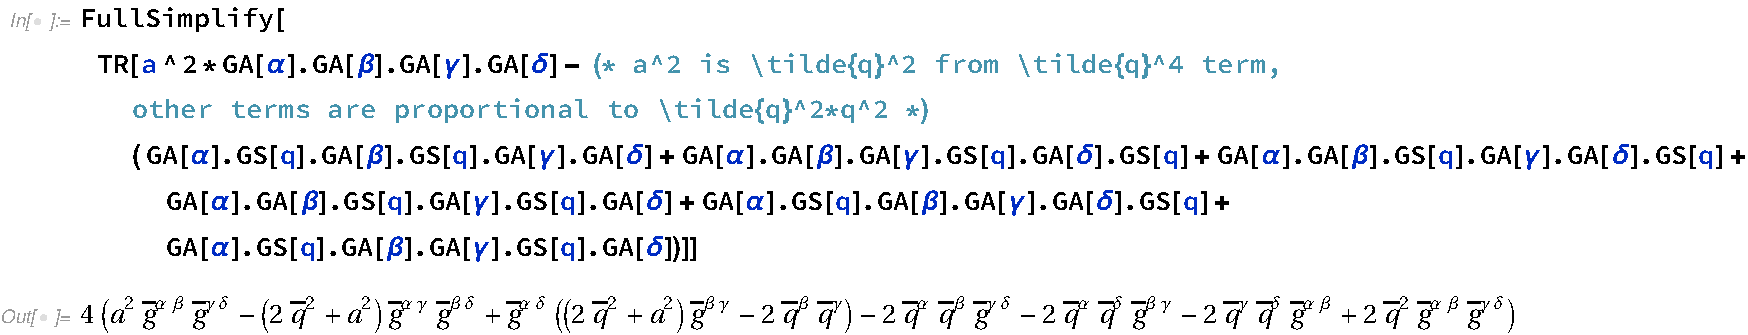
\includegraphics[width=1.0\textwidth]{Figures/Trace_4ptfct_Mathematica}
  \end{center}
  \setlength{\belowcaptionskip}{-20pt}
  \caption*{}
\end{figure} \\
As usual we plug this in the definition of $R_2$ and evaluate the integrals to get the expression of $R_2$ for the first of the contributing diagrams.
\begin{align*}
R_2 = & \frac{1}{\left( 2\pi \right) ^4} \int d^d\bar{q} \frac{\tilde{N}}{\bar{D}_0 \bar{D}_1 \bar{D}_2} = \frac{1}{\left( 2\pi \right) ^4} \int d^d\bar{q} \frac{4e^4}{\bar{D}_1 \bar{D}_{13} \bar{D}_2 \bar{0}} \tilde{q}^2 \lbr \left( 2q^2 + \tilde{q}^2 \right) \left( g^{\alpha\delta}g^{\beta\gamma} - g^{\alpha\gamma}g^{\beta\delta} + g^{\alpha\beta}g^{\gamma\delta} \right) + \right. & \\
& \left. - 2 \left( g^{\alpha\beta}q^{\gamma}q^{\delta} + g^{\gamma\delta}q^{\alpha}q^{\beta} + g^{\alpha\delta}q^{\beta}q^{\gamma} + g^{\beta\gamma}q^{\alpha}q^{\delta} \right) \rbr = & \\
& = \frac{-4e^4}{\left( 2\pi \right) ^4} \lbr \left( 2 \left( \frac{-i\pi^2}{3} \right) + \left( \frac{-i\pi^2}{6} \right) \right) \left( g^{\alpha\delta}g^{\beta\gamma} - g^{\alpha\gamma}g^{\beta\delta} + g^{\alpha\beta}g^{\gamma\delta} \right) - 2 \left( \frac{-i\pi^2}{12} \right) \left( g^{\alpha\beta}g^{\gamma\delta} + g^{\gamma\delta}g^{\alpha\beta} + \right. \right. & \\
& \left. \left. + g^{\alpha\delta}g^{\beta\gamma} + g^{\beta\gamma}g^{\alpha\delta} \right) \rbr = \frac{ie^4}{4\pi^2} \lbr \frac{5}{6} \left( g^{\alpha\delta}g^{\beta\gamma} - g^{\alpha\gamma}g^{\beta\delta} + g^{\alpha\beta}g^{\gamma\delta} \right) - \frac{1}{6} \left( 2 g^{\alpha\beta}g^{\gamma\delta} + 2g^{\alpha\delta}g^{\beta\gamma} +  \right) \rbr = & \\
& = \frac{ie^4}{24 \pi^2} \left( 3 g^{\alpha\beta}g^{\gamma\delta} - 5 g^{\alpha\gamma}g^{\beta\delta} + 3 g^{\beta\gamma}g^{\alpha\delta} \right) &
\end{align*}

\begin{align*}
R_2^{4\gamma} = & 2 \left[ R_2 + R_2 \left( \alpha \leftrightarrow \delta \right) + R_2 \left( \alpha \leftrightarrow \beta \right) \right] = \frac{2ie^4}{24 \pi^2} \lbr \left( 3 g^{\alpha\beta}g^{\gamma\delta} - 5 g^{\alpha\gamma}g^{\beta\delta} + 3 g^{\beta\gamma}g^{\alpha\delta} \right) + \left( 3 g^{\beta\delta}g^{\alpha\gamma} - 5 g^{\gamma\delta}g^{\alpha\beta} + 3 g^{\beta\gamma}g^{\alpha\delta} \right) + \right. & \\
& \left. + \left( 3 g^{\alpha\beta}g^{\gamma\delta} - 5 g^{\beta\gamma}g^{\alpha\delta} + 3 g^{\alpha\gamma}g^{\beta\delta} \right) \rbr = \frac{ie^4}{12 \pi^2} \left( g^{\alpha\beta}g^{\gamma\delta} + g^{\alpha\gamma}g^{\beta\delta} + g^{\beta\gamma}g^{\alpha\delta} \right) & \numberthis \label{eqn:R24photon}
\end{align*}

Like the other 3-point function all of the other 4-point functions which are permitted by the Feynman rules vanish. We will not show this here because the calculations for the 4-point functions are quite lengthy.